\documentclass[iop,apj]{emulateapj}
\usepackage{amsmath, amssymb, amstext}
\usepackage{todonotes}
\usepackage[breaklinks, colorlinks, citecolor=blue, linkcolor=magenta]{hyperref} 
\renewcommand*{\sectionautorefname}{Section}
\usepackage[all]{hypcap}
\usepackage{aas_macros}
\usepackage{natbib}
%\linespread{2.5}
\bibliographystyle{apj}
\shorttitle{Short Title}
\shortauthors{Author et al.}
\begin{document}

\title{Detecting Active Asteroids/Comets from OSSOS survey images}
\author{Authors}
\affil{Affiliations}

\begin{abstract}
Abstract.
\end{abstract}

\keywords{keywords}
\maketitle

\section{Introduction}

Until the last decade, comets and asteroids have been thought of as separate populations differing both in morphology and dynamics. With different fractions of volatile content, an obvious differentiator is the presence of a transient coma and/or tail, whereas asteroids exhibit bare nuclei photometric properties. [fill in: mention Tisserand parameter here?]  With the recent advent of large wide-field surveys which have regularly monitored large populations of solar system objects, objects which exist between the classification of comets and asteroids have been identified in steady numbers. The classical view of comets being primarily icy bodies with highly eccentric orbits, and asteroids being primarily rocky bodies with stable orbits confined to the main asteroid belt between Mars and Jupiter \citep{sheppard14}, has been usurped by the discovery of comet-asteroid transition objects. With the discovery of asteroids in dynamically cometary orbits, dynamically asteroidal objects that exhibit burst of cometary activity or are associated with meteor streams such as the Damocloids (\cite{sonnett11}; and references therein, \cite{gilbert09}) the classification criteria for asteroids and comets has become less obvious. Objects such as these may be comets which have exhausted their volatile content or are dormant, or asteroids which have a higher volatile fraction. In this study we focus on the `active asteroids' (AAs) (or main belt comets (MBCs)), which are a population of bodies with stable asteroid-like main belt orbits that exhibit transient comae or tails consistent with cometary morphology.  As it is expected that objects which are in the inner solar system would have long ago sublimated their ice away, the active asteroids pose an interesting insight to the heliocentric distance at which ice condenses, known as the `snow line', which of interest to planetary formation and determining the chemistry of the early solar nebula.

%The active asteroids are small bodies in the main asteroid belt which have transient dust emission producing comet-like comae and tails. Unlike comets, which originate in the Kuiper Belt and Oort cloud, and have been scattered inwards by gravitational effects, the active asteroids have stable orbits confined to the main belt and likely formed in the same location as they reside presently \citep{sheppard14} \citep{fernandez02}. 
% A standard criterion for interpreting the differing dynamics between the comet and asteroid populations is the Tisserand parameter, with respect to Jupiter, where comets have a value less than three, and asteroids greater than three.  It has been observed that asteroids may have comet-like orbits \citep{gilbert09} (and references within) and there are also objects with cometary properties in asteroid-like orbits (active asteroids or main belt comets). Since the discovery of these intermediate type objects, the classification criteria for asteroids and comets has become less obvious.

For objects which formed in the the outer region of the main belt, the crystallized water ice which was present at the time of formation and not exposed to primordial heating may still remain in reservoirs beneath the surface \citep{prailnik09}.  According to models developed by \citet*{fanale89},  beyond heliocentric distances of 2.4 AU ice can be protected against sublimation by a relatively thin surface regolith  of depth 1 -- 100 m for the entire age of the solar system. If the ice layer were to be exposed to sub solar heating,  sublimation could be triggered which would  eject dust particles from the surface producing a coma [todo: check that wording not too similar to paper]. The source of the dust emission may be different for each object and could include ice sublimation, impact ejecta, rotational instabilities due to YORP torques, or a combination of several effects. (\cite{hsieh15}; and references therein).  

% impacts inferred from observed large brightening and quick fading 
% sublimation inferred from prolonged or periodic activity during perihelion passage, Hsieh et al 2010, 2011
%The ejected dust would form a coma around the object, and radiation pressure affects would then (preferentially) push the smaller particles away from the asteroid forming a tail.
%Sublimation driven active asteroids differ from comets in that the comets, having larger ice reservoirs, would have stronger sublimation events which could eject larger debris. The cometary tail would then be longer lived as the larger debris would be less effected by the radiation pressure, and thus dissipate slowly. It is also possible, however, that prolonged activity is a result of ongoing ejection of small, fast dissipating particles. \cite{TEST} 

Since the first discovery of an active main-belt asteroid, 133P/Elst-Pizarro \citep{elst96}, several attempts have been made to identify new objects of this type; at present, eighteen objects have been identified (Figure 1) [todo: check figure reference] \citep{jewitt15}. A comprehensive review of these surveys can be found in \citet{hsieh15}.  A persistent challenge to this effort is that the detection of the faint coma or tails around small dark objects is highly dependent on the magnitude constraints of the survey. As most asteroids fall near the limiting magnitude of the survey in which they are discovered [todo: citation necessary?], objects which are larger, closer, or have higher albedo are preferentially detected and any dust emission would be more easily apparent. At present, the active fraction of identified active asteroids greater than 1 km to main belt asteroids greater than 1 km is $f \, \sim \, 10^5$, and describes a strong lower limit as many objects are yet undetected. \citep{jewitt15} %From a study of 30,000 objects observed near perihelion, \cite{} Hsieh et all (2015) concluded that $f \, \sim \, 10^4$ for asteroids which are active at any instant in the outer belt.

In this paper, we present a study using the Canada-France-Hawaii Telescope (CFHT) Outer Solar System Origins Survey (OSSOS) data to identify the presence of cometary activity in previously discovered asteroids. We select the Hungaria family as the test group for our search pipeline. Previously undetectable emission activity may be able to be identified in the OSSOS survey, which was designed to detect trans neptunian objects and as such has a limiting magnitude that is much lower than previous surveys \citep{hsieh15}. The survey covers a wide field of both the ecliptic plane and low inclinations allowing for the observation of a large number of main belt objects in different orbital phase spaces. In this study we
identify all observations of previously discovered main belt objects in the OSSOS data set, and identify potential activity by measuring the asteroidal brightness profile and comparing this to a stellar model profile in order to detect a large deviation in width potentially characteristic of a coma or jet around the asteroid. This is similar to the process employed by \citet*{luu92} and \citet*{sonnett11}.

% From the results of both methods we compute upper limits for the expected number of active asteroids.


\section{Observations}

Observations taken by OSSOS with the CFHT MegaPrime wide-field optical imaging facility  at the summit of Mauna Kea, Hawaii, have been collected since 2013. The wide-field imager, MegaCam, consists of a 36 CCD image plane, each 2048 x 4125 CCD with resolution of 0.185"/pix. This covers a field of  roughly 1$^{\circ}$ x 1$^{\circ}$ on the sky. Each block of data taken consists of a mosaic of 21 segments of one-square-degree sky coverage, and at present, covers two orbital phase spaces on the plane of the ecliptic, and two off plane at low inclinations. The OSSOS survey employs the u* and r' filters on the MegaCam with integration times of 287, 387, and 500 seconds, yielding a lower limit of 24.5 magnitudes.

% how is the image data calibrated? filters, S/N? MOPS?
The OSSOS images are reduced via the moving object pipeline (MOP). [todo: how reduced]. (standard data detrending???) Source characteristic measurements were obtained from source extraction \citep{sep} and were used to extract the orbital information the transient object. 


%As the identified active asteroids do not share a specific phase space the analysis was not constrained to just the main belt or plane of the ecliptic, but for all known objects with heliocentric distances beyond the inner belt (a \textgreater \, 2.064 AU), inclinations below 40$^{\circ}$, and eccentricity less than 0.45. 
% to detect objects in the main asteroid belt, objects with semimajor axis 2.064 < a < 3.277 AU, e < 0.45, i < 40 deg
% PSF detections
% cuts, identifying process

\section{Analysis}

From the calculated arcs provided by SSOIS \citep{ssois} of main belt objects in the AstDys catalogue \citep{astdys} we were able to predict which asteroids were present in the OSSOS data set and could be examined for cometary activity. From a set of 3528 images, there are [todo: fill in] observations of [todo: fill in] asteroids in the OSSOS data. We analyze a small group of objects in the Hungaria family as our test case for our automated pipeline. Of the 1187 Hungarias we have 76 observations of 25 objects. 

\subsection{Object identification}

An automated pipeline was written to identify each asteroid in an OSSOS exposure by: it's location relative to the predicted coordinates,  elongation due to trailing effects caused by the apparent rate of motion over the duration of the exposure, and apparent magnitude. 

The coordinates of each object in the exposure were obtained from the photometric software \citep{sep}, and objects which were closest to the predicted location (at the midpoint of the exposure) as calculated by known arc \citep{jpl} [todo: is this citation necessary?] were chosen as candidate objects. If no objects were detected within a set radius calculated from the uncertainty in the asteroid arc, the radius was increased by a factor of 1.5.

The expected elongation of the trail was calculated from the predicted motion of the asteroid over the length of the exposure \citep{jpl} under the assumption of constant motion. This value was then compared to the elliptical shape parameters measued by the photometry of each candidate object. 
A difficulty in this process is that objects which are moving faster during the exposure, and thus trailed to a greater extent, will not be elliptical in shape. As the photometry is optimized for point sources and extended sources such as galaxies, the accuracy of the shape parameters, and thus the astrometry, is correlated to the extent of the elongation. For this reason we implement an error of 20 percent on the measurement of the semi-major and semi-minor axis of the elliptical shape parameters reported by the photometry. 

The inability of the photometry software to correctly measure the shape of the asteroid trail will also have an effect on the measured flux as the aperture may not include the total amount of light. As the centre of the object is determined by the flux weighted barycenter of the object, this may also result in an inaccurate measurement of the astrometry. In order to avoid this error, the centre coordinates of the object were chosen as the centre of the elliptical aperture for fast-moving objects. 
In addition, the elongation effect in itself may effect the accuracy of the flux measurement without taking into account the potential loss of light. This is a result of the flux being spread over a larger area than the point spread function (PSF), which reduces the per unit area apparent magnitude and the signal-to-noise \citep{veres12}. A direct consequence is a lowered limiting magnitude for fast moving asteroids. 
A third consideration is that objects which are active and have jets or a coma will appear brighter than the expected magnitude calculated from previous observations. Depending on the extent of the activity, this could cause the object to be measured as several magnitudes greater than predicted. For this reason we did not exclude objects which were bright than expected.  
Therefore, in subjecting the candidate object to a consistency check with the predicted value, we used an uncertainty of at least 2 magnitudes, and did not reject the object if it was inconsistent. Instead we maintained a record of which object passed which consistency checks with the intent of reviewing visually those that passed further tests based on their accuracy with respect to the expected values. 
 
An candidate object which did not meet any of the criteria mentioned about would be rejected. This would include objects which were involved with or too close to bad pixels or cosmic rays, on the edge of the CCD, in a diffraction ring of a nearby bright star, or that could not be accurately measured by the photometry software.

In order to accurately measure the PSF of the asteroid -- which is necessary to check for anomalous flux surrounding the object that could indicate activity -- it is necessary to ensure that the asteroid is isolated from other sources. This involvement check was preformed with a comparison of a catalogue of bright sources built for the OSSOS images \citep{ossos} in the region surrounding the asteroid, and the cases where the asteroid was involved were rejected.

Applying this identification process left 49 exposures of 19 asteroids to be examined.

\begin{table}[htdp]
\caption{caption goes here}
\begin{center}
\begin{tabular}{lc}
	\textbf{Rejection cause}								& 	\textbf{\# images} \\
	\hline
	Involved with background stars                                     	& 	1			\\
	Incorrectly resolved as two objects					& 	5			\\
	Did not meet elongation or magnitude criteria			& 	2			\\
	Incorrectly measured by the photometry				& 	5			\\
	Could not be processed by the photometry software	& 	6			\\
	Off the edge of the CCD								& 	5			\\
	In saturated region of nearby bright star				& 	2			\\
	Could not be resolved from the background 			&	1			\\
	\hline
	Retained											& 49       
\end{tabular}
\end{center}
\label{default}
\end{table}

\subsection{PSF comparison}

A postage stamp of size 2.5 times the full-width-half-maximum (FWHM) and centred on the midpoint of the elongated shape was rotated such that asteroid trail was aligned parallel to the pixel rows on the CCD chip. The asteroid profile was averaged over the entire length of the postage stamp. The stellar model PSF was built from the OSSOS MOP at the location of the asteroid on the CCD to account for any distortion, and rotated by the same angle.  The profile was measured as the average over the width of the model star. A 3 sigma difference between the subtracted profiles was used to indicate the presence of additional flux around an asteroid, characteristic of a cometary comae. There were [fill in] asteroids which were measured to be above this limit and were flagged for visual confirmation. Due to saturation effects, asteroids with magnitudes greater than 18.5 were not analyzed for activity. However, as previous surveys have included this set of objects \citep{hsieh15} we were comfortable with this exclusion.

\subsection{Detection Efficiency}

How well do we identify coma vs jets vs tails ? How may do we detect vs observed? What are the statistics? Why are the results so bad?

\section{Discussion}

As the involvement check was preformed using a catalogue of bright objects, it is possible that some asteroids identified and carried through the pipeline process were involved with dim background objects. An example of this is shown in figure 3. Depending on the geometry of the involvement this could be selected as an asteroid with activity, possibly a large bright jet. In order to distinguish between activity and involvement, the asteroids with unusual PSF's were all manually reviewed. Through this process we could determine whether a jet was present, in which case the outflowing dust would also have a trailing effect through the exposure, or if it were a case of involvement. We do not expect that a jet would be present for a fraction of the exposure time during one observation. 

\section{Recommendations }

Use a trail fitting function for improved photometry on fast moving objects such as described by \cite{veres12}.
Tail detection pipeline like \cite{sonnett11}

\acknowledgments{
  Acknowledgments. 
}

%  Authors SHOULD NOT be listed alphabetically
\bibliographystyle{plainnat}
\bibliography{mbc_paper}

% to be updated when the new get_iamges for all objects in families has been completed
\begin{figure}[!htb]
    \centering
    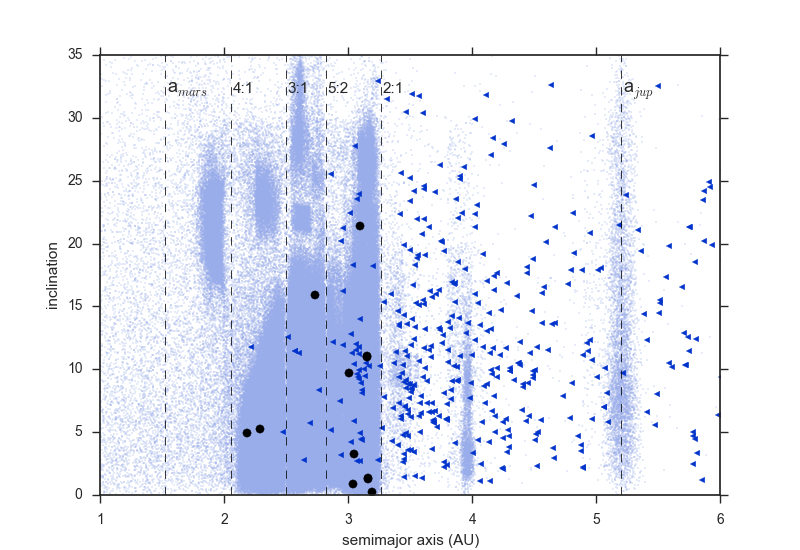
\includegraphics[height=9cm]{graphs/aa_comets_mba_all.png}
    \caption{Inclination of all known objects in the main asteroid belt as a function of semimajor axis.  Mean motion resonances between Mars and Jupiter as well as the planet's semimajor axis are marked in dashed lines, main belt objects are marked as light small dots, comets as arrows, and active asteroids as stars. \cite{mpc}}\label{fig:1}
\end{figure}

%\begin{figure}[!htb]
%    \centering
%    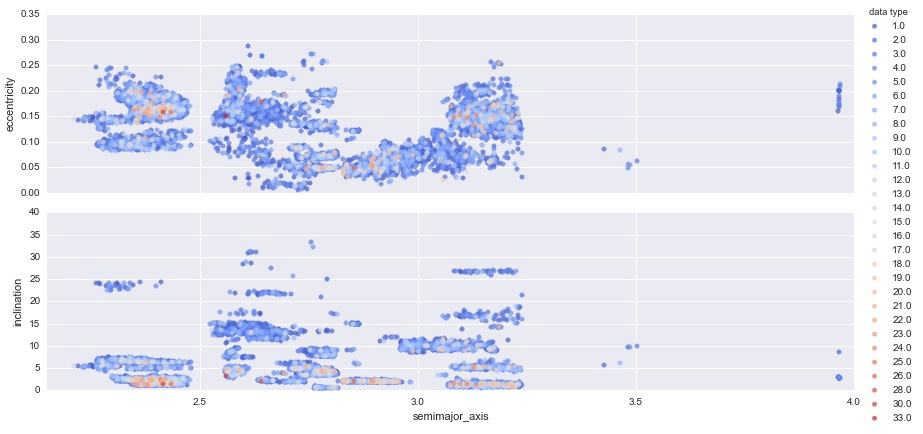
\includegraphics[height=7cm]{graphs/a_e_i_occur.png}
%    \caption{Inclination and eccentricity as a function of semi-major axis of all objects. Colours represents number of observations (occurrences) used in the analysis}\label{fig:2}
%\end{figure}
%
%\begin{figure}[!htb]
 %   \centering
%    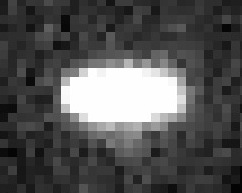
\includegraphics[height=4cm]{images/background_gal.jpeg}
%    \caption{An asteroid involved with a dim background object. }\label{fig:3}
%\end{figure}


\end{document}



